\chapter{Methods}\label{chapter:method}

{ \color{red}

    about 10-30 pages (rather more I guess)

    \begin{itemize}
        \item (1/3 of thesis)
        \item start with a theoretical approach, describe the developed system/algorithm/method from a high-level point of view,
        \item go ahead in presenting your developments in more detail
        \item make sure to not refer to results section too much. rather leave info out if it cannot explained well without looking at the results
    \end{itemize}
}

\section{Causal Model}
In essence, our analysis combines causal methods for data generation and ground-truth feature attribution. 
The main process is intervening on a hyperparameter such as the later discussed coupling ratio $\rho$, then training models and using them to generate predictions and explanations. 
Within this greater structure, a subprocess generates the images used for training with a structural causal model, taking only $\rho$ as an input. While $\rho$ stays fixed for a single instance of data generation, it is a causal variable in the overarching model. 

\subsection{Data Generating Causal Model}
For the most exact comparison of attribution between a model and its explanation it is imperative to know the ground truth of the training data. A structural causal model (SCM) can define variables and the \textit{independent} mechanisms with which they interact precisely. We want to define an SCM that closely mirrors image generation processes as they happen in realistic scenarios. 
Explicitly using a generating SCM has previously been done to create or test new attribution methods \cite{Parafita2019, Wilming2023,Clark2023, Goyal2019, Reimers2019, Reimers2020}. A few other works evaluating XAI methods with a known ground truth have implicitly used structures akin to an SCM without defining it in causal language \cite{Kim2018, Yang2019,Arras2022}. 

The causal graph and its structural assignments used for our experiment are defined as follows: 
\begin{align}
&G:=\eta^g &\mathrm{with} \  \eta^g \sim \mathcal{N}(0.5,0.02) && \notag \\ 
&N_w:=\eta^w &\mathrm{with} \  \eta^w \sim \mathcal{N}(0.5,0.1) && \notag \\ 
&N_s:=\eta^s &\mathrm{with} \  \eta^s \sim \mathcal{N}(0.5,0.1) && \notag \\ 
&N_x:=\eta^x &\mathrm{with} \  \eta^x \sim \mathcal{N}(0,0.05) && \notag \\ 
&W:=(\rho * G + (1-\rho)* N_w) \geq 0.5 \notag \\ 
&S:=(\rho * G + (1-\rho)* N_s) \geq 0.5 \notag \\ 
&Z:= U(0,245760)
& \mathcal{X} = W + f_{image}(S, Z) + N_{x} &
\end{align}

\begin{figure}[H]
    \centering
    \includegraphics[width=0.9\textwidth]{pics/generating_scm.png}
    \caption[Data Generating SCM]{Data Generating Structural causal model.
        $\rho$ is not explicitly visible in the SCM. It determines the signal-to-noise ratio between the confounding $G$ and the noise variables $N_w$ and $N_s$. The noise terms of $Z$ and $G$ are not shown explicitly.}
    \label{fig:generating_scm}
\end{figure}

The SCM as seen in \cref{fig:generating_scm} and \cref{eq:scm} serves as a ground truth for our experiment. It is mostly an additive model using Gaussian distributions for the noise terms, except for $Z$ (uniform noise) and the not further specified function generating the images out of the latent factors.

The meta-variable $\rho$ adjusts how much information is shared between the true class information (shape), which we name \textit{core feature} following \cite{Singla2022} and the watermark or \textit{spurious feature} through a shared common ancestor named generator $G$. For each model/data combination coupling $\rho$ is fixed, to later enable a comparison between models trained with different coupling ratios. \\

A second parameter which we keep fixed for all experiments, determines how frequent the spurious feature is in the data. We set this parameter which could be termed \textit{prevalence} to 0.5, so that just as many images have a watermark as not. It is important to note that this particular SCM is just one of many possible ways to model how spurious features might interact with core features. It attempts to follow the logic of how images are generated or selected in real datasets. Here, it particularly looks at pathways for the generation of \textit{Clever-Hans} or \textit{watermark} features, often present in image datasets \cite{Lapuschkin2019}. As visible in \cref{fig:equivalent_scm} different causal models can produce an equivalent distribution of the two latent factors in question (watermark and shape). One can think of more variations of SCMs which are able to produce the same correlation, so the choice of using the confounder version as in \cref{fig:generating_scm} is mainly due to its ease of implementation. Without assumptions about the generating mechanism, the confounder case is not identifiable, i.e. distinguishable, from $W \rightarrow G \rightarrow S$ and $S \rightarrow G \rightarrow W$ because it is Markov equivalent to those scenarios. 
Although the presented collider case (\cref{fig:generating_scm}\textbf{a}) is theoretically distinguishable from the confounder case (\textbf{b}), one can not hope that a network which only has access to the intervened on (selected) data will recover this. 

The idea of investigating the effect of a coupling ratio $\rho$ was inspired by Wilming et al. \cite{Wilming2023}, who also used a \textit{signal-to-noise} ratio in their generating model. Instead of a confounding model their learned data instances are colliders of the label and a suppressor variable. The expected explanation importance of this suppressor feature therefore ought to be zero, as long as the collider is not intervened on. We contest this assumption, as it is not clear whether a neural network does not implicitly create interventions on this collider (which is the image set), therefore introducing correlation between the parent components through a selection bias. 

The direction of causal links for image classification is highly debatable and shall not be the focus of this work. Whether the selection of the AI researcher reducing costs with free images resulted in classes being polluted with watermarks (\cref{fig:equivalent_scm}\textbf{a}), or whether a scientist marked x-rays with their diagnosis (\cref{fig:equivalent_scm}\textbf{b}) is indistinguishable for ML models. 
Instead, we only want to find to what degree a neural network learns, and attribution method explains the distribution generated by a particular SCM.

To evaluate the results of the current experiment and see how having a different SCM might influence the outcome we will later look at other generating SCMs too (\cref{chapter:results}).

\begin{figure}[H]
    \centering
    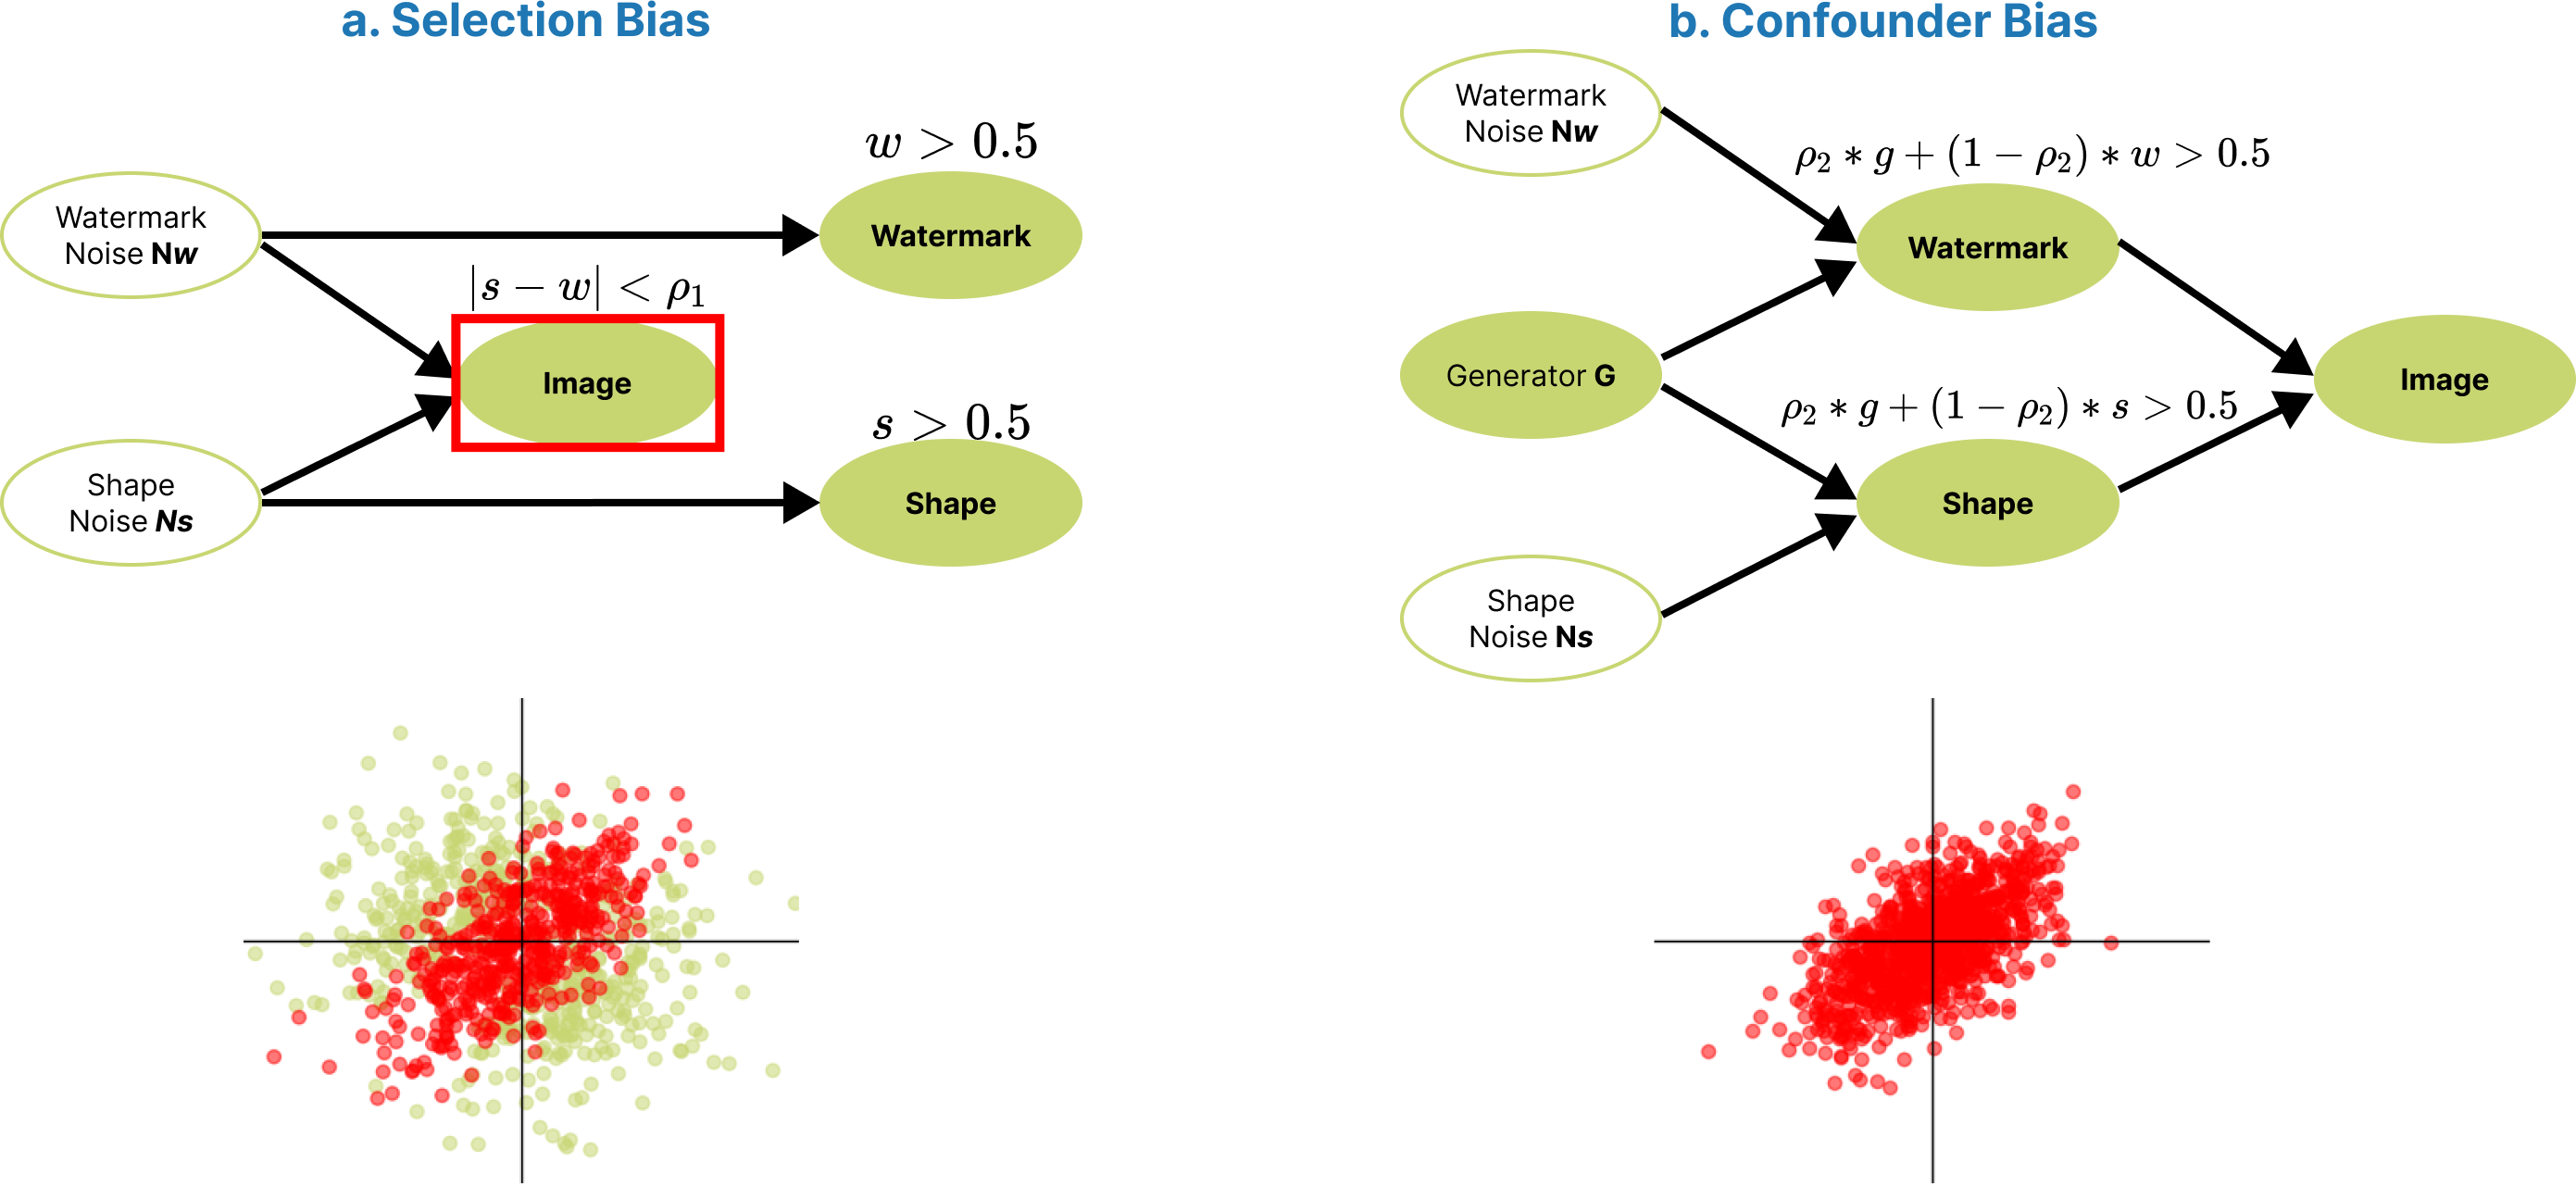
\includegraphics[width=0.8\textwidth]{pics/equivalent_scm.png}
    \caption[Selection vs. Confounder Bias]{SCMs typically found in image datasets.
    \textbf{a.} Selection Bias \textit{(researcher chooses images from free online collection with watermarks)}
    \textbf{b.} Confounder Bias \textit{(e.g. scientist marks positive x-ray scans with sign)}}
    \label{fig:equivalent_scm}
\end{figure}

\subsection{Explanation Generating Model}
The data generation causal model is part of the model which generates predictions and explanations.
This model is defined in a similar way to the \textit{explanation generating process (EGP)} in Karimi et al. \cite{Karimi2023}.
Ratio $\rho$ is a meta-variable of our image generation process in a similar sense to how hyperparameters are defined for the training there. While \cref{fig:generating_scm} depicts the data generating causal model (DGCM) of the training dataset in more detail, \cref{fig:egp} shows how this is embedded into the mechanism of generating explanations. 

\begin{figure}[H]
    \centering
    \tikzset{%
        neuron/.style={
                circle,
                draw,
                minimum size=8mm
            }
    }
    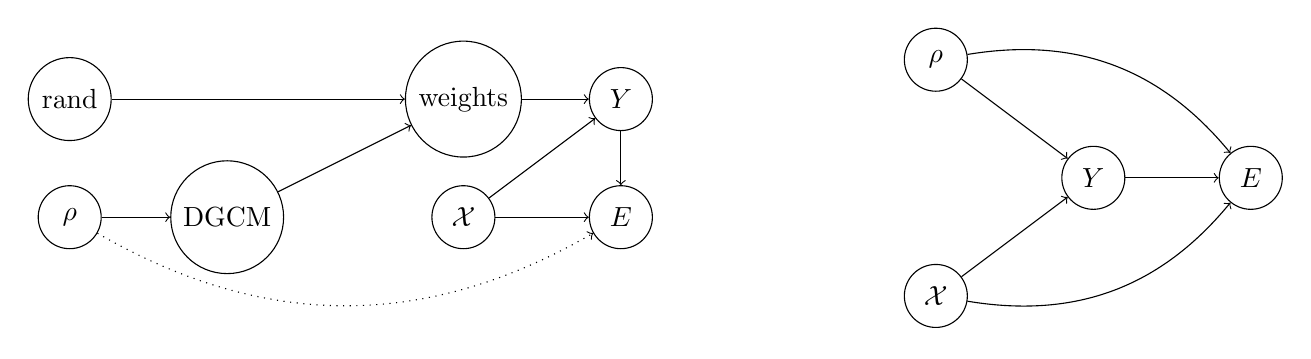
\begin{tikzpicture}[every node/.style={ draw, minimum size=8mm, align=center},]

    % generating model:
        \node [neuron]  (r) at (0.0,1) {$\rho$};
        \node [neuron]  (rs) at (0,2.5) {rand};
        \node [neuron]  (scm) at (2,1) {DGCM};
        \node [neuron]  (ws) at (5,2.5) {weights};
        \node [neuron]  (x) at (5,1) {$\mathcal{X}$};
        \node [neuron]  (p) at (7,2.5) {$Y$};
        \node [neuron]  (e) at (7,1) {$E$};

        \draw[->] (r) -- (scm);
        \draw[->] (rs) -- (ws);
        \draw[->] (scm) to (ws);
        \draw[->] (ws) -- (p);
        \draw[->] (x) -- (p);
        \draw[->] (x) -- (e);
        \draw[->] (p) -- (e);
        \draw[->, bend right=30, dotted] (r) to (e);
        
    % simplified causal model:
        \node [neuron]  (r) at (11,3) {$\rho$};
        \node [neuron]  (x) at (11,0) {$\mathcal{X}$};
        \node [neuron]  (p) at (13,1.5) {$Y$};
        \node [neuron]  (e) at (15,1.5) {$E$};

        \draw[->] (r) -- (p);
        \draw[->] (x) -- (p);
        \draw[->, bend right=30] (x) to (e);
        \draw[->] (p) -- (e);
        \draw[->, bend left=30] (r) to (e);
    \end{tikzpicture}
    \caption[Explanation Generation Process (EGP)]{Explanation Generation Process \textit{EGP} (left), Simplified Causal Model (right)}
    \label{fig:egp}
\end{figure}

\subsection{Watermark Benchmark Dataset W-dSprites}\label{section:causal_model}
Although this thesis is not the first work to use a toy dataset with known generating factors to evaluate attribution methods, we aim to find a new dataset which is as simple as possible and yet mirrors the main workings of a realistic computer vision problem. For this we adapted the dSprites dataset \cite{dsprites17} by adding small watermarks in the shape of '\textit{w}'s to some images. The dSprites dataset was originally constructed as a means for testing the degree of disentanglement a machine learning model has achieved. It contains images with rectangles, ellipses or hearts in varying positions, scales and rotations. To simplify the task more we only use the rectangle and ellipse class for our experiment. Another motive is that in a binary classification task positive and negative relevance might be used in varying strategies for prediction. In theory this could make the class-insensitivity studied by Sixt et al. \cite{Sixt2020} visible or counteract it. Further details can be found in the appendix \cref{appendix:dsprites}.

\begin{figure}[H]
    \centering
    \includegraphics[width=0.6\textwidth]{pics/dsprites_examples.png}
    \caption[Example Images W-dSprites]{First row: images from the original dSprites dataset, second row: images from the W-dSprites dataset with small \textit{w} as a watermark on some images in random positions at the edge of the image and Gaussian noise added.}
    \label{fig:dsprites_examples}
\end{figure}

\section{Generating Explanations with Concept Relevance Propagation}
The previously described causal framework can be applied to a multitude of explanation methods as it is principally model- and method-agnostic. However we limit our analysis to CRP, its predecessor LRP and interpretation techniques constructed with CRP.
Producing explanations using concept relevance propagation requires decisions on the backpropagation rule(s), on the conditioning sets and potentially further hyperparameters. 
We follow the recommendations or default settings of CRP's authors \cite{Achtibat2022, Achtibat2023} and best practices \cite{Kohlbrenner2020} as closely as possible.
For the backpropagation we apply the $LRP_{\varepsilon -z^+- b^-}$ - rule as recommended by \cite{Kohlbrenner2020}. Due to the simplicity of our CNN model no more model canonization steps need to be applied. See \cref{appendix:lrprules} for further technical details. 

\begin{figure}
    \centering
    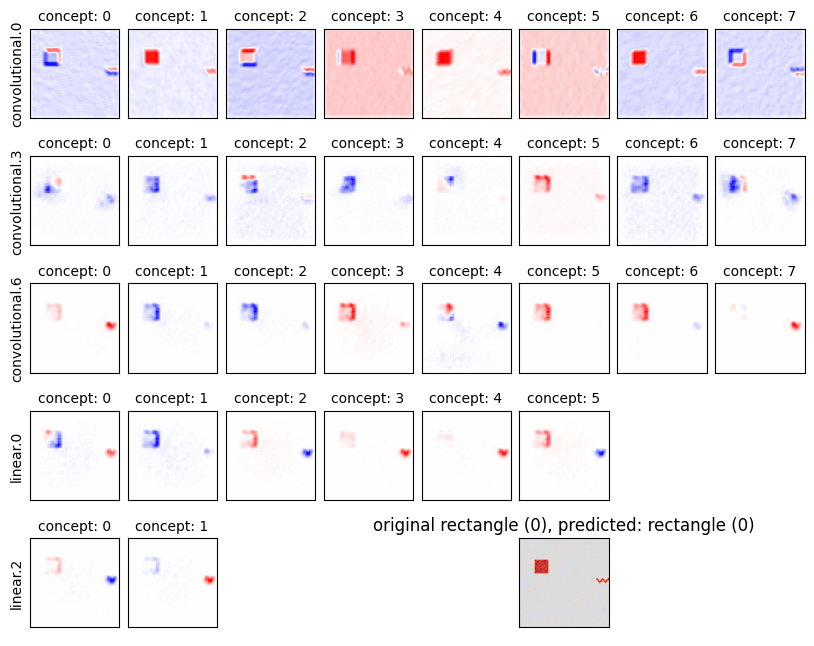
\includegraphics[width=0.8\textwidth]{thesis_latex_template/pics/conditional_heatmaps.png}
    \caption[Comparing Attribution Maps of Layers]{Concept-conditional heatmaps for one example image. Note the Sobel-filter-like attributions in earlier layers and the more combined attributions of watermark and shape in later layers.}
    \label{fig:cc_heatmaps}
\end{figure}

Principally, neurons in every layer of a model can be conditioned on using the CRP-approach. However, the resulting attribution maps are not necessarily depicting disentangled and abstract enough concepts. When looking at a \textit{concept-conditional} attribution maps from the earlier layers, one will likely see low-level features. In the later fully connected layers before the output the potentially disentangled concepts might get mixed together again for the final decision. In \cref{fig:cc_heatmaps} an example shows the tendency from trivial to abstract \textit{concepts}. 
According to \cite{Dreyer2023a, Zeiler2013} the last convolutional layer is ``most likely representing disentangled representation''. For comparison we investigate both the last convolutional (layer 3) and the first fully connected layer (layer 4) of the 5 total layers. It is not entirely clear whether the extremely small size of our model hinders a transfer of the results to realistic scenarios. Yet training significantly larger models would have been too computationally expensive for this approach. \\

In the following we will reiterate the steps necessary to produce multiple types of explanations with CRP:

\subsubsection{Concept-Conditional Attribution Maps and Relevance for Prediction}
The concept-conditional backpropagation rule described in \cref{section:crp_background} can be applied to arbitrary sets of neurons $\theta$. In our scenario we create class-specific attribution maps conditioned on each neuron in the selected layer (3 or 4). For this we use the output for the predicted class as the initialization for relevance, keep all other layers untouched and then mask out the other neurons relevance in the layer $\ell$. 
\begin{equation}
    R_{i}^{\ell}(\mathrm{x} |\theta_{\ell}=\{i\}) 
\end{equation}
Backpropagating all the way to the input yields an attribution map $R_i^{\ell}$, however the relevance $r_i$ assigned to the neuron in question from previous layers can be used as an approximation of its overall importance for the prediction.

\begin{itemize}
    \item should I keep class the same or change per instance?
    \item Should I really do everything both for last convolutional and first fully-connected layer?
\end{itemize}

\subsubsection{Local Concept Importance}
Masking the desired region in the image and computing attributions for this area. (is kinda the same as just taking importance in that area???, but then normalized with their recommended method)


{\color{gray} \subsubsection{Relevance Maximization}
To arrive at reference sets of the neurons in our selected layer, relevance maximization finds images that maximize concept-conditional relevance. As mentioned by \cite{Achtibat2022} using the whole dataset might make the selected images too similar to each other. Hence we compute the maximization for a subset of 1000 images to enforce more variance. Importantly, the sample we select from does not have the association between $S$ and $W$, meaning that watermarks are equally likely to occur on rectangle as on ellipse images. 
The implementation provided by CRPs authors produces sets of 40 images for each neuron in each layer. 

\subsubsection{Perceptive Field}
Information on the concentration of the relevance within the images selected for each concept can be gained by applying concept localization. Following the approach of \cite{Yeh2020} and using tools from the existing LRP toolset \cite{Anders2023} Achtibat et al. visualize only the part of the selected images that contributed to the neurons activation. 
The implementation of this and all previously described methods is made accessible by CRPs authors at \url{https://github.com/rachtibat/zennit-crp}.
}


\section{Data Ground Truth Correlation $m_0$}
The goal of this analysis it to gather information on how a known coupling ratio of two features interacts with their importance to the model and their explained importance. 
Measure $m_0 = \rho$ is the correlation between the shape and watermark feature in our data generating model. When $\rho$ is 0, the features are not associated at all, when it is 1 they correlate perfectly. Conceived as a \textit{signal-to-noise} ratio between the correlated and uncorrelated parts of $S$ and $W$, it can directly be used as a measure of the coupling of spurious (watermark) and core (shape) feature. However the data generating process introduces a small offset due to the binarization of the variables $W$ and $S$. It might therefore be more insightful to look at the actual correlation of the features in the generated data distribution as a ground-truth. This is also sensible because we only sample a small subset from the data generating SCM  for training and can not expect the distribution to perfectly align with $\rho$. Considering that we have two binary variables their correlation can be measured using the $\phi$-coefficient. It is also called \textit{Matthews} or \textit{Yule phi} coefficient and can be interpreted like the Pearson correlation coefficient for two binary variables:

\vspace{1em}
\begin{minipage}[t]{0.45\textwidth}
\begin{tabular}{|c|c|c|c|}
    \hline
     & y= 1 & y = 0 & total  \\  \hline
    x= 1 & $n_{11}$ & $n_{10}$ & $n_{1*}$ \\ \hline
    x= 0 & $n_{01}$ & $n_{00}$ & $n_{0*}$ \\ \hline
    total& $n_{*1}$ & $n_{*0}$ & $n$ \\ \hline
\end{tabular}
\end{minipage}%
\begin{minipage}[c]{0.45\textwidth}
\begin{align}
& \phi = \frac{n_{11} * n_{00} - n_{10}*n_{01}}{\sqrt{n_{1*}*n_{0*}*n_{*0}*n_{*1}}}
\end{align}
\end{minipage}
\vspace{1em}

Generally, we do not want and neither expect the model to perfectly reconstruct $\rho$ or the data correlation $\phi$. After all, the strength of neural networks presumably lies in recovering the truly important feature even when other, highly correlated features are present. Though some research expects explanations to give insight into the distributions of the training data to better understand how biases might occur, even if a model has apparently learned to ignore spurious features \cite{Kindermans2017}. 

\begin{figure}
    \centering
    \includegraphics[width=0.5\textwidth]{thesis_latex_template/pics/gt_m0_phi_only.png}
    \caption[Choosing measure for $m_0$]{$\rho$ plotted against $\phi$-coefficient of sampled training data distributions }
    \label{fig:finding_rho}
\end{figure}

\section{Establishing a Ground-Truth Model Feature Importance $m_1$}\label{section:gt_measure}
In contrast to realistic application scenarios our causal framework enables us to establish the ground truth importance of features for a trained model. Similar to recent work on causal attribution \cite{Goyal2019,Parafita2019,Karimi2023} the causal effect of an intervention upstream on the output of a model can be estimated in the following way:
\begin{center}
Average Causal Effect of latent factor $W$ on output $Y$ \\
\begin{equation}
\displaystyle ACE = \mathbb{E} [ Y \ | \ do(W=1) ] - \mathbb{E} [ Y \ | \ do(W=0) ] 
\end{equation}
\end{center}
The intervention on a given latent factor is straight-forward here, as our factors of interest are both binary variables (watermark and shape). Due to our knowledge of the ground truth we can condition on all other latent factors and feed one image with the watermark and the same image without it through the neural network. Thereby achieving a pure intervention on our $W$.  
However it is not naturally clear how to define the output of a neural network. One can either measure the average causal effect on the binary prediction or on the output layers' logits, which change in a continuous fashion.
To account for the effect of the initialization of model weights and biases on the usage of either feature, we average each measure over multiple random seeds (see \cref{fig:gt_over_seeds}).

\subsection{Prediction Flip}
Computing the Prediction Flip is straight forward in our example as we can control all variables. 
This binary causal effect can be estimated as the percentage of images for which the prediction flips, when the factor is flipped, which in turn is equivalent to the $\phi$-coefficient between prediction $Y$ and watermark $W$ (see proof in \cref{appendix:phi_equals_pf}). Therefore this measure is apt for the comparison with the $W,S$ correlation in the training data distribution.

We expect this variant of the model importance to be less sensitive to the spurious watermark feature $W$. The reason being, that while the continuous output vector (i.e. \textit{confidence}) might already be affected by the spurious feature for weaker biases, the prediction will only flip once the spurious feature becomes more important than the core feature. For example, an image without a watermark might be correctly classified as an ellipse, but the same image with the watermark might have a higher activation for that class.

For better readability we will refer to an image with the watermark $\mathrm{x}_{do(W=1)}$ as $\mathrm{x}$ and the same image without the watermark $\mathrm{x}_{do(W=0)}$ as $\mathrm{x}'$ in the future.
\begin{equation}
\displaystyle 
PF =\frac{1}{|\mathcal{X}|} \sum_{\mathrm{x} \in \mathcal{X}} |y(\mathrm{x}) - y(\mathrm{x}') |
\end{equation}


\subsection{Mean Logit Change}
For the W-dSprites classification task, the output vector consists of 2 logits $y_0$ and $y_1$. The model predicts \textit{rectangle} when $y_0 > y_1$ and \textit{ellipse} otherwise. To compute the mean logit change when intervening on our watermark spurious feature $x$, we take a sufficient amount of samples $\mathcal{X}$ from our dataset and feed them through the model. First we predict images with $W=1$ (containing a watermark) then with $W=0$. It is important to choose a reasonable distance measure between the two output vectors. \cite{Sixt2022a} and \cite{Goyal2019} use the mean absolute difference. To enable better comparison we use the soft-max confidences as during the training process. This keeps the relative magnitudes within the sample set intact but brings it to the range $[0,1]$. All measures are scaled so that the distance for maximally different instances is 1, which in this case means dividing by 2. Although we compute the euclidean distance for the explanations later, this is not necessary here, as for 2D vectors $D_{euclid} = \sqrt{D_{abs}}$.\\

Mean Absolute Difference:
\begin{align}\displaystyle 
& \MLC_{\rho, m}^{abs} = \frac{1}{|\mathcal{X}| * 2} \sum_{\mathrm{x} \in \mathcal{X}} 
|y_0(\mathrm{x}) -y_0(\mathrm{x}')| + |y_1(\mathrm{x}) -y_1(\mathrm{x}')| 
\end{align}

Recently, assessing the similarity of per-concept relevances has also been done using the cosine similarity \cite{Sixt2020, Achtibat2022}. Therefore we also include the cosine distance as a potential metric for the model importance $m_1$. We are not convinced that this metric has properties we seek for evaluating logits of a network as it does not exhibit triangle inequality cite?.  
\begin{align}\displaystyle 
& \MLC_{\rho, m}^{cosine} = \frac{1}{|\mathcal{X}|}\sum_{\mathrm{x} \in \mathcal{X}}  
1 - \frac{\vec{y}(\mathrm{x}) \cdot \vec{y}(\mathrm{x}')}
{\lVert \vec{y}(\mathrm{x}) \rVert \lVert \vec{y}(\mathrm{x}')\rVert }
\end{align}


\section{CRP Explanation Importance $m_2$}\label{section:measure}
Our goal is to compare the causal effect of an upstream intervention on the true feature importance and then the explained feature importance. After having defined multiple ways to measure the models true feature importance, we need to repeat the process for the explanation produced by CRP. It is not well known how humans perceive changes in an explanation and there is no agreed upon scale of importance, so we believe it is best to construct multiple measures to test against each other. {\color{gray} Additionally, the authors of CRP introduce multiple interpretation techniques using this method which potentially enable better human understanding. }Most of the proposed metrics are derived from existing work on evaluating feature importance in XAI \cite{Sixt2020, Karimi2023, Arras2022} \\

Each candidate should be a variation of measuring the effect of intervening on $W$ on an explanation:
\begin{center}
Average Causal Effect of latent factor $W$ on explanation $e$: \\
\begin{equation}
\displaystyle ACE = \mathbb{E} [e \ | \ do(W=1) ] - \mathbb{E} [ e \ | \ do(W=0) ]
\end{equation}
\end{center}
The core question is, whether the influence on the explanation of changing $\rho$ is completely mediated by our prediction. A perfect explanation assigns just as much importance to a feature as the model and does not depend on other factors. This is one way to describe the fidelity of the explanation to the model. The proposed measures however try to incorporate other notions of goodness applied for XAI such as \textit{intelligibility} and especially \textit{complexity}. \\

The measures introduced in the following are roughly ordered from measures being most true to the numerical effect of intervention on the explanation to measures reducing the complexity of the explanation to what is understood. Although human perception is not part of our evaluation, aiming for less complex explanations seems to be more in line with a \textit{good} explanation. While the first measure would require the user to compare multiple heatmaps pixel-wise to find differences, later metrics use only one pixel or a reduced (hopefully more human-understandable) concept. \\

Many related works remove negative relevances in attribution maps to enable comparison with XAI methods that do not measure negative relevance. Another reason could be that incautious aggregation of negative and positive relevance could introduce cancelling-out effects. We believe, however, that a spurious feature can be negatively as well as positively attributed for a model to be biased. In a complex network, we cannot be sure that there are no neurons purely negatively associating a feature with one class. Therefore the measures mostly equally incorporate both the magnitude of the positive and negative relevance. 


\subsection{Mean Attribution Change}
The likely most straight-forward way to calculate explanation importance for neurons in a layer using CRP is to measure the average causal effect of an intervention on the attributions directly. This approach aims to emulate the \textit{mean logit change} of the prediction for the concept-based explanation. In a given layer $\ell \in L$, the relevance of each of the neurons $i in \ell$ for the overall prediction is used. As in \cite{Achtibat2022}, the relevances for the neurons are scaled to sum to 1 and are interpreted as relative importance percentages.
Also, the attributions for each of the $|\ell|$ neurons in $|\ell|$ concept-conditional heatmaps is computed using CRP.

We compute the neurons relevance and their attribution map with the CRP method the following way:
\begin{align*}
& r_i(\mathrm{x}) = R(i | \theta=\{y\}) \\
& R_i^{\ell}(\mathrm{x}) = R(\mathrm{x} | \theta=\{i, y\}) \\
\end{align*}

The causal effect of intervening on the spurious watermark feature on one neuron is then the difference between its attribution map of one image with a watermark and the same image without a watermark. If the model has indeed learned distinct concepts for each feature, the same effect should also become visible, when just looking at the relevance values for each neuron in a layer.\\

To look at the difference in explanation, multiple distance metrics could be applied. We compare multiple types of dissimilarity between the two heatmaps (i.e. 2-dimensional pixel maps). Firstly, we look at the mean absolute pixel-wise difference. The Euclidean distance seems the second natural approach. Because we compute the \textit{cosine distance} for the relevance values $r_i$ as proposed by the authors of CRP \cite{Achtibat2023}, we also compute the measure for the attribution maps for completeness.
Lastly, we measure the kernelized treatment effect which Karimi et al. also use in their experiment \cite{Karimi2023}. \\ 

A sensible normalization for a set of attribution maps is not as trivial as for the output vector or the relevance vector. The naive approach would be again, to take the maximally opposing images difference. But it is not to be expected that any method would assign large positive or negative values to every pixel. Instead, the results of attribution methods only sparsely assign attribution to few pixels, usually within regions of objects and not to the background. 
We therefore have to find a smaller divisor which scales a maximal difference between an image with and without watermark to approximately 1.
To adjust for the sparsity of the attributions, we take the maximal sum of absolute values of all heatmaps sampled for one model. This \textit{maximal absolute sum} scaling is similar to what Achtibat et al. \cite{Achtibat2022} apply to the relevances of a layer to interpret them as (positive or negative) percentage values.\\

Here we show the different possible distance metrics for the attribution maps.
\begin{align}
\displaystyle 
& r_{tot}(\mathrm{x}) = \sum_{i \in \ell} \sum_{p \in P_x} 
|R_{p,i}(\mathrm{x})| \notag \\
& \max_{\rho, m}^E = \max_{\mathrm{x} \in \mathcal{X}} (r_{tot}(\mathrm{x}) , \  r_{tot}(\mathrm{x}') ) \notag \\
& \MAC_{\rho, m, \mathrm{x}}^{abs} = 
\sum_{i \in \ell} \sum_{p \in P_x} |R_{p,i}(\mathrm{x}) -R_{p,i}(\mathrm{x}')|* \frac{1}{\max_{\rho, m}^E} \\
& \MAC_{\rho, m, \mathrm{x}}^{euclid} = \sqrt{ \sum_{i \in \ell} 
\sum_{p \in P_x}\left(\frac{R_{p,i}(\mathrm{x}) -R_{p,i}(\mathrm{x}')}{\max_{\rho, m}^E}\right)^2
} \\
& \MAC_{\rho, m,\mathrm{x}}^{cosine} =
\frac{R(\mathrm{x}) \cdot R(\mathrm{x}') }{|R(\mathrm{x})|\cdot |R(\mathrm{x}')|} \\
& \MAC_{\rho, m, \mathrm{x}}^{kernel} = k(R(x) ,R(x) ) + 2 k(R(x) ,R(x') ) + k(R(x') ,R(x') )  
\end{align}

Once a distance metric is chosen, we need to aggregate results over all sample images, and then again over the models initialized with different seeds.

\begin{align}
& \frac{1}{|M_\rho|\cdot |\mathcal{X}| }\sum_{m}^{M_{\rho}} \sum_{\mathrm{x,x'}}^{\mathcal{X}} Metric(\mathrm{x,x'})
\end{align}

The pixel-wise relevance should be assigned to different attribution maps proportionally to the total relevance over the different neurons of the layer, but it might still be reasonable to weigh the per-neuron distance with its absolute relevance $r_i$. The reason being, that high variation in unused or unimportant neurons might distort the overall distance, while there are less differences in the important pixels and vice-versa:

\begin{align}
& \frac{1}{|M_\rho|\cdot |\mathcal{X}| }\sum_{m}^{M_{\rho}} \sum_{\mathrm{x,x'}}^{\mathcal{X}} \sum_{i in \ell} 
Metric(\mathrm{x,x'}, i) * |r_i(\mathrm{x})|
\end{align}

Although this (possibly weighted) difference is constructed to measure the causal effect of intervention on the explanation as closely as possible, it ignores one of the core ideas of concept-based and local attribution methods potential usefulness. If adding or removing a watermark has a significant effect on some pixels far away from it, this is not in line with desirable properties of a good explanation such as interpretability or even fidelity to the ground truth importance. It is likely that through the coupling of watermark and shape in our experiment, the changes of relevance do not only affect the watermark region itself but at least the shapes importance too. 
Another potential downfall for human intuition is the way more localized concepts are attributed in comparison to more global or wide-spread concepts. Achtibat et al. \cite{Achtibat2022} show an example where the eye of a dog wrongly seems to be more important than its fur in a general attribution map, because it is concentrated on a smaller region. A similar thing can potentially happen with our experiments watermark, as it fills a small region in comparison to the larger shape feature. 

In the \cref{section:region_specific} we thus introduce measures which concentrate on the attributed relevance within the ground-truth region and relative to the rest of the attribution map.
We also further reduce the estimation of whether a concept (i.e. filter) encodes the spurious watermark feature or something else. 

\subsection{Concept Relevance Vectors}
Without looking at the attribution maps it is still interesting to see whether the total relevance of certain neurons changes when intervening on the watermark $W$ or the shape $S$ feature. If the neural network indeed follows different strategies when the watermark is present versus when it is not, then different concepts should be relevant depending on the features value. 
In contrast to previous measures, this measure is not computed in the attribution map space, but only in the relevance space. We therefore have no information on which concepts the filters encode, only how important they are. Achtibat et al. still look at concept relevances extensively as they assume them to encode human-understandable concepts. While for the previous measures the aim was to extract the importance from the visual explanation, for this measure we only assume that different filters should be at work depending on the presence of the watermark, if it has significance.
We find it necessary to make this distinction: A filter could change strongly when intervening on the watermark. But if this change (or the importance of the watermark for that filter) is not visible from the attribution maps, it is impossible to decipher which concept that filter encodes without access to ground-truth concepts. 

For the relevances within a layer, we apply the same distance metrics as described in the previous section except that summing over pixels is not necessary. Also, the relevances are already in a $[-1,1]$ interval and sum up to maximally 1 per image due to the recommended normalization. The resulting distances however can range up to 2 because of possible negative relevances, hence we divide the effect sizes by 2 to facilitate comparison. 

\subsection{Importance in Ground-Truth Region}\label{section:region_specific}
In \cite{Arras2022} two metrics for the analysis of importance in pixel maps are introduced. Relevance Mass Accuracy (RMA) measures the ratio of relevance within a bounding box around a feature to the total relevance. Relevance Rank Accuracy (RRA) rates the percentage of pixels in such a bounding box that fall within the $k$ most important pixels in the heatmap. If those metrics are accurately describing the relative importance of a feature for the explanation too, they should be applicable in our experiment. 

\subsubsection{Relevance Mass Accuracy (RMA)}
When trying to establish whether a feature is important, one would intuitively look at that feature first. Therefore approaches like Relevance Mass Accuracy take into account the known boundary of a feature for benchmarks with ground-truth importance. Luckily, in our benchmark dataset the shape and watermark feature are spatially separated so this strategy is applicable.
Bau et al. \cite{Bau2017, Bau2020} have defined a similar measure to compare an explanation importance to a ground truth, which they term IoU (from \textit{Intersection over Union}). Both these works assume the perfect attribution of importance to one feature to be a binary mask, which is 1 inside and 0 outside the features region. \\
As noted in \cite{Arras2022} it is not known whether this perfect score is attainable or even desirable for an explanation. Yet the overall tendency should become clear.

For our localized metric we apply a strategy resembling these evaluation scores. 
Fortunately, the authors of CRP have already formulated \textit{local concept importance}, evaluating the conditional attribution to a concept in a predefined region by masking the rest of the attribution map out. 
While RMA in the CLEVR-XAI benchmark uses the exact pixel-boundary of an object, we use a bounding box around the watermark \textit{w}. This is because the small model we apply smoothes out relevance over a region due to pooling layers in the model. \\

\begin{figure}
\begin{minipage}[t]{0.45\textwidth}
    \vspace{-\topskip}
        \includegraphics[width=\textwidth]{thesis_latex_template/pics/bounding_box.png}
\end{minipage}
\begin{minipage}[t]{0.45\textwidth}
    \begin{align}\displaystyle
    & R_B(\mathrm{x}) = \sum_{p_x \in B} R_{p_x}(\mathrm{x} | \theta)\\
    & RMA(\mathrm{x}) = \frac{R_B(\mathrm{x})}{R(\mathrm{x})}
    \end{align}
\end{minipage}
\caption{Bounding Box $B$ around watermark}
\label{fig:bounding_box}
\end{figure}

The \textit{localized relevance score} is the amount of conditional relevance attributed to a certain region of an image. In our case, the region of interest are pixels in the bounding box $B$ around the watermark (see \cref{fig:bounding_box}. 

To enable better comparison we again embed this measure within the watermark/no watermark effect estimation setting, even though we do not expect an image without a watermark to apply any relevance within the bounding box.

Albeit this approach is reducing complexity, it has been noted that importance is hard to gauge when features have varying spatial extends. \cite{Achtibat2022} points to an example where the fur of a dog actually has larger total relevance but in the heatmap the snout seems to be more important because its attribution is more concentrated. A similar thing could happen with the watermark feature because it is usually smaller than the shape itself. 
To potentially combat this, we set the relevance within the bounding box in relation to the total relevance, which yields the RMA score.
While this metric might give us a good estimate of the actual relevance of the watermark, the heatmap could still produce a wrong understanding of relative relevance for humans. \\

\subsubsection{Relevance Rank Accuracy (RRA)}
The second metric adapted from \cite{Arras2022} is \textit{Relevance Rank Accuracy}.  
Relevance Rank Accuracy orders the input features (i.e. pixels) by relevance and finds the $k$ most relevant pixels. The rank $k$ is equal to the size of the region of the feature, in question, here the bounding box around the watermark. Computing the ratio of the top-k relevant pixels inside of the bounding box $B$ to $k$ yields \textit{Relevance Rank Accuracy}:

\begin{align*}
& P_{top-k} = (p_1, p_2,...,p_k | |R_{p_1}| > |R_{p_2}| > ... > |R_{p_k}| ) \\
& RRA(\mathrm{x}) = \frac{|P_{top-k} \cap B|_\mathrm{x}}{|B|} 
\end{align*}

Arguably, this metric loses even more information on whether at least some importance is assigned to the spurious feature (watermark). Previous work has also pointed out many issues with this or similar methods. However it reduces the complexity of the explanation by only looking at the k-most important pixels. \\

\subsubsection{Pointing Game}
A step towards even more reduced complexity is the \textit{Pointing Game} metric, first introduced in \cite{Zhang2016}. The only difference between RRA and the Pointing Game metric is, that the latter \textit{binarizes} the question whether a feature is important by setting $k = 1$. If the most important pixel is inside the watermark bounding box $B$, the watermark is important, otherwise not.
We can then use this information as a binary weight on the relevances of concepts. 
It has been noted by others that the pointing game metric is sub-optimal for evaluating attribution maps, as pointing to the central pixel in an image already produces ''good'' results. However, as our watermark changes position on the sides of the image and is quite localized, we think that this measure can still function as an approximation. 

These metrics are all defined for one general heatmap and we have to find a generalization for $|\ell|$ attribution maps for the filters in a layer. Just summing up the values for all concepts would not generate a useful result as the relative relevance of each filter is removed from these region-specific measures. Instead, we create a weighted sum of the scores over the neurons. As weights we use the absolute relevances $|r_i|$ to potentially incorporate negative relevance of the spurious feature too. 

\section{Direct vs. Indirect Influence of $\rho$}
After having computed a ground truth effect of $m_0 = \rho$ on the feature importance (of the watermark feature $W$) and the effect on the explanation, we can compare them.
While a visual comparison of the curves of importance might award us a first impression, measures like mutual information, correlation can be applied to give us real insights. 
In general it is not clear which type of relationship (linear, non-linear) to expect between $m_0, m_1, $ and $m_2$. Therefore the methods we can apply to test the independence of $E$ on $\rho$ given $Y$ are only an approximation and not definite.

\begin{figure}
    \centering
    \includegraphics[width=0.8\textwidth]{thesis_latex_template/pics/gt_m0_m1.png}
    \caption[$m_0$ vs. $m_1$]{Comparing $\phi$-correlation coefficient (blue) and mutual information (MI) (red) between shape and watermark for subset of 6400 images. \\ \textit{dashed}: true label biased data distribution, \textit{dotted}: prediction for biased data distribution \textit{solid}: prediction for unbiased data distribution }
    \label{fig:m0_m1}
\end{figure}

In \cref{fig:m0_m1} the relationship between our causal variable and the coupling within the datasets becomes visible, while the relationship to what the model has learned is not as \textit{linear}. The most concerning result would be, if the explanation had an even weaker relationship with $\rho$ than the prediction. That would be mean that the explanation is not able to recover spurious features sufficiently. 

Here we need to expand on exactly which methods we apply to compare the effects on prediction vs explanation. 

Karimi: Compare effect of Rho on Y and Rho on E with correlation analysis. Then randomly permute predictions Y, Compute Explanations E thereof. Again perform correlation analysis Rho,Y,E. 
use performance buckets with control group either within each performance bucket or use same accross all buckets. 
We have to do it differently here.

Easiest: 
- MSE or similar distance metric
- correlation (Pearson???)
- something that encodes correlation but penalizes, if measures scales differ to strongly (i.e. they increase proportionally, but the one reaches 1, the other only 0.2)


\section{CNN Model Zoo}\label{section:training}
To evaluate explanations, the model to test on can neither be to simple and therefore easy to explain, nor too large and therefore an overkill for the simple dataset at hand.
Through a simple trial-and-error search the architecture detailed in \autoref{lst:cnnmodel} with 3 convolutional layers of 8 channels, one fully connected \textit{concept} layer with 6 neurons and finally the fully connected output layer was deemed most fitting for the task. While less convolutional channels or layers often resulted in the model not converging at all, having more neurons or potentially \textit{concepts} did not seem to add information but just redundancy.
This model reliably yields test accuracies over 90\% when using the same feature distribution $\rho$ as used for training. As stated before, we fix all hyperparameters, as they are not part of this analysis, to values produced from a short search.
The only hyperparameter we deemed necessary to control for, is the random initialization of weights and biases. In preliminary experiments it became clear that some seeds react profoundly differently to $\rho$ than others. For example, one instance is able to ignore the watermark even when it is perfectly correlated with the shape ($\rho = 1$), while others easily change their strategy to predict from this spurious feature (see \cref{fig:gt_over_seeds}). The ground-truth importance and the general performance of these models seem to not correlate at all, differently to what Karimi et al. observe \cite{Karimi2023}.
For further information on hyperparameters and training, refer to \cref{appendix:model}

\begin{figure}
    \centering
    \includegraphics[width=\textwidth]{thesis_latex_template/pics/compare_seeds.png}
    \caption[Comparing Seeds]{Prediction Flip ($\phi$-coefficient between prediction and watermark) over 16 random seeds}
    \label{fig:gt_over_seeds}
\end{figure}

{\color{codepurple} 
\textbf{Notation}:
\begin{enumerate}
    \item Image instances $:= \mathcal{X}$, one image $:= \mathrm{x}$
    \item pixels in image $\mathcal{X} := p_x$
    \item Watermark variable $:= W$ value for variable $:= w$
    \item bounding box of watermark $:= B$
    \item Shape variable/ label $:= S$ value for shape $:= s$
    \item coupling ratio $:= \rho$
    \item prediction $:= P$
    \item explanation variable $:= E$ single instance of explanation $:= e$
    \item Layer set $:= L$, Layer in neural Network $:= \ell$ neuron in layer $:= i$
    \item other factors $:= Z$ single factor $:z_i$ \\ 
    \textit{enumerate: scale, rotation, posX, posY}
    \item (Gaussian) noise terms for each causal var $:= N_{variable}$
    \item Random Seed number $:= M (=10)$, one seed/ index $:=m$
\end{enumerate}
}